\documentclass{ctexart}

\usepackage{amsmath}

\usepackage{amsthm}

\usepackage{amssymb}

\usepackage{bm}

\usepackage{graphicx}

\usepackage{listings}
\lstset{
basicstyle=\scriptsize
}

\usepackage{caption}

\begin{titlepage}

\title{微分方程数值解 \\ 第十四周作业}

\author{于慧倩 \\ 14300180118}

\date{2017年6月}
\end{titlepage}

\begin{document}

\maketitle

\newpage

\begin{enumerate}

\item P222.2

跳蛙格式:

$$
\frac{u_i^{n+1}-u_i^{n-1}}{2 \tau}+c \frac{u_{i+1}^n-u_{i-1}^n}{2h}=f_i^n
$$

\begin{enumerate}

\item 截断误差

\begin{eqnarray*}
R_{i+1} &=& \frac{u(t_{n+1},x_i)-u(t_{n-1},x_i)}{2 \tau}+c\frac{u(t_n,x_{i+1})-u(t_n,x_{i-1})}{2h}-f(t_n,x_i)\\
&=& \frac{u(t_{n+1},x_i)-u(t_{n-1},x_i)}{2 \tau}+c\frac{u(t_n,x_{i+1})-u(t_n,x_{i-1})}{2h}\\
&&-\frac{\partial u(t_n,x_i)}{\partial t}-c\frac{\partial u(t_n,x_i)}{\partial x}\\
&=& \frac{u(t_{n+1},x_i)-u(t_{n-1},x_i)}{2 \tau}-\frac{\partial u(t_n,x_i)}{\partial t}\\
&&+c\frac{u(t_n,x_{i+1})-u(t_n,x_{i-1})}{2h}-c\frac{\partial u(t_n,x_i)}{\partial x}\\
&=& R_t+R_x
\end{eqnarray*}

\begin{eqnarray*}
R_t&=& \frac{u(t_{n+1},x_i)-u(t_{n-1},x_i)}{2 \tau}-\frac{\partial u(t_n,x_i)}{\partial t}\\
&=& \frac{\tau^2}{3!} \frac{\partial u(t-n,x_i)}{\partial t} +O(\tau^2)
\end{eqnarray*}

\begin{eqnarray*}
R_x&=& c \frac{u(t_n,x_{i+1})-u(t_n,x_{i-1})}{2 h}-\frac{\partial u(t_n,x_i)}{\partial x}\\
&=& c\frac{h^2}{3!} \frac{\partial u(t-n,x_i)}{\partial x} +O(h^2)
\end{eqnarray*}

\begin{eqnarray*}
R_{i+1}&=&R_t+R_x\\
&=&\frac{\tau^2}{3!} \frac{\partial u(t-n,x_i)}{\partial t}+ c\frac{h^2}{3!} \frac{\partial u(t-n,x_i)}{\partial x} +O(\tau^2) +O(h^2)
\end{eqnarray*}

\item 数值稳定性

利用传播因子法估计

代入$u_i^n=g(n)e^{i \omega x_i}$得

$$c  
\frac{g(n+1)-g(n-1)}{2 \tau}e^{i \omega x_i}+c\frac{g(n)e^{i \omega x_{i+1}}-g(n)e^{i \omega x_{i-1}}}{2h}=0
$$

两边提取$e^{i \omega x_i}$得
$$
\frac{g(n+1)-g(n-1)}{2 \tau}+cg(n)\frac{e^{i \omega h}-e^{-i \omega h}}{2h}=0
$$
$$
\frac{g(n+1)-g(n-1)}{2 \tau}+cg(n)\frac{i \mbox{sin} \omega h}{h}=0
$$

令$\lambda = i \displaystyle \frac{c \mbox{sin} \omega h}{h},\lambda^2<0$,则增长因子满足

$$
G^2-1+2 \tau \lambda G=0
$$

\begin{enumerate}
\item $\tau^2 \lambda^2 +1\geq 0$时

$$G = -\tau \lambda \pm \sqrt{\tau^2 \lambda^2 +1}$$

$$|G|^2 = \tau^2 |\lambda|^2 +\tau^2 \lambda^2 +1=1$$


\item 选取$\omega$使得 $\tau^2 \lambda^2 +1 < 0$时

$$G = -\tau \lambda \pm i \sqrt{-\tau^2 \lambda^2 -1} $$

$$|G|^2 = (-\tau |\lambda|\pm \sqrt{-\tau^2 \lambda^2 -1})^2  $$

可以选取$\omega$对应的某个根的模$|G|>1+\frac{c\tau}{h}$,这时不稳定。

总之,可以选出$\omega$使得格式不稳定,所以格式不稳定。


\end{enumerate}
\end{enumerate}


\item P222.5 取初值为方波时,考虑$X=2,T=1$的总体情况,$c=1$所以迎风格式取左偏格式。


\begin{enumerate}


\item 初值为第一种时,无论$r=1,r=1/2$都是稳定的,作出下图:

\centerline{\includegraphics[width=5in]{trian.eps}}


\item $r=1$时

三种格式都退化成$u_{i}^{n+1}=u_{i-1}^n$,取$X=2,T=1$时,作出下图:

\centerline{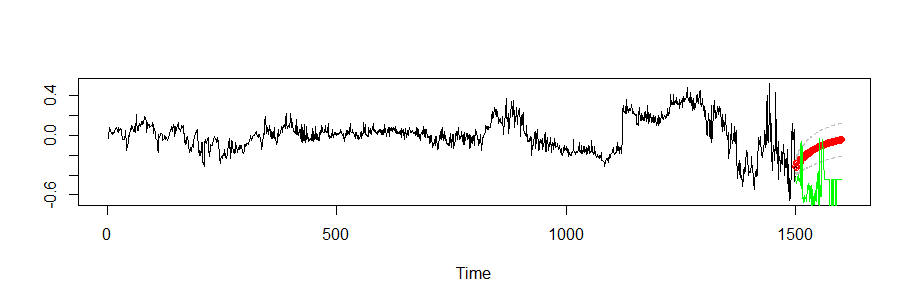
\includegraphics[width=5in]{11.eps}}



\item $r=\frac{1}{2}$时候

$T=1$时三种方法得到的解:

\centerline{\includegraphics[width=5in]{bijiao.eps}}

分别作出精确值、迎风格式、Lax格式、Lax-Wendroff格式如下:

\centerline{\includegraphics[width=5in]{exact1.eps}}

\centerline{\includegraphics[width=5in]{uy1.eps}}

\centerline{\includegraphics[width=5in]{ulax.eps}}

\centerline{\includegraphics[width=5in]{ulw.eps}}

\end{enumerate}



\end{enumerate}
\end{document}
















